\documentclass{article}
\usepackage[utf8]{inputenc}
\usepackage{tikz}
\usetikzlibrary{automata}

\title{State Diagram for Markov Chain}
\author{Tarandeep Singh}
\date{January 2022}

\begin{document}

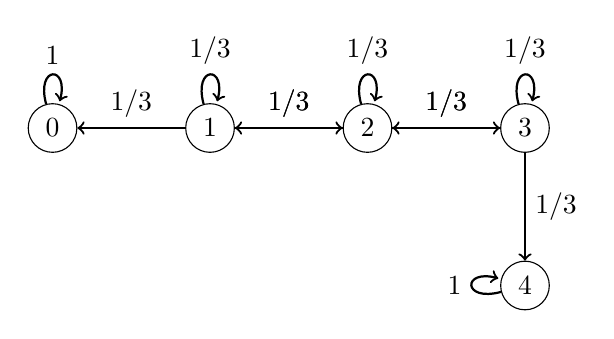
\begin{tikzpicture}

\tikzstyle{vertex} = [circle,draw=black]
\tikzstyle{edge} = [->,thick]

\node[vertex](v1) at (0,0){0};
\node[vertex](v2) at (2,0){1};
\node[vertex](v3) at (4,0){2};
\node[vertex](v4) at (6,0){3};
\node[vertex](v5) at (6,-2){4};

\draw[edge] (v1) edge[loop above] node{1} (v1);
\draw[edge] (v2) -- node[above]{1/3} (v1);

\draw[edge] (v2) edge[loop above] node{1/3} (v2);
\draw[edge] (v2) -- node[above]{1/3} (v3);
\draw[edge] (v3) -- node[above]{1/3} (v2);
\draw[edge] (v3) edge[loop above] node{1/3} (v3);
\draw[edge] (v3) -- node[above]{1/3} (v4);

\draw[edge] (v4) -- node[above]{1/3} (v3);
\draw[edge] (v4) edge[loop above] node{1/3} (v4);
\draw[edge] (v4) -- node[right]{1/3} (v5);

\draw[edge] (v5) edge[loop left] node{1} (v5);

\end{tikzpicture}

\end{document}